%%%%%%%%%%%%%%%%%%%%%%%%%%%%%%%%%%%%%%%%%%%%%%%%%%%%%%%%%%%%%%%%%%%%%%%%%%%%%%%%%%
\begin{frame}[fragile]\frametitle{}
\begin{center}
{\Large Introduction}
\end{center}
\end{frame}


%%%%%%%%%%%%%%%%%%%%%%%%%%%%%%%%%%%%%%%%%%%%%%%%%%%%%%%%%%%%%%%%%%%%%%%%%%%%%%%%%%
\begin{frame}\frametitle{A graph is}
{\emph \ldots a set of discrete objects, each of which has some set of relationships with the other objects}

Abstraction:

\begin{center}
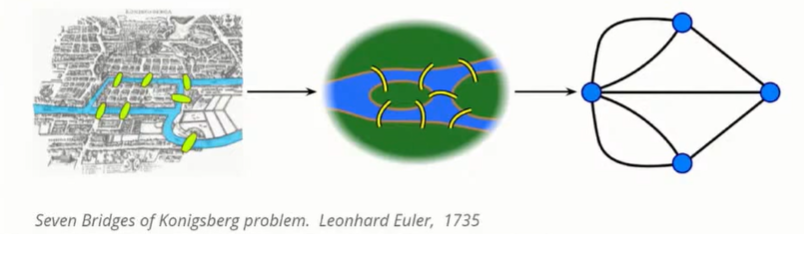
\includegraphics[width=\linewidth,keepaspectratio]{neo4j4}
\end{center}	  

{\tiny (Ref: Introduction to Neo4j - a hands-on crash course - neo4j)}
\end{frame}

%%%%%%%%%%%%%%%%%%%%%%%%%%%%%%%%%%%%%%%%%%%%%%%%%%%%%%%%%%%
\begin{frame}[fragile]\frametitle{ Graph-structured Data Are Ubiquitous }

\begin{center}
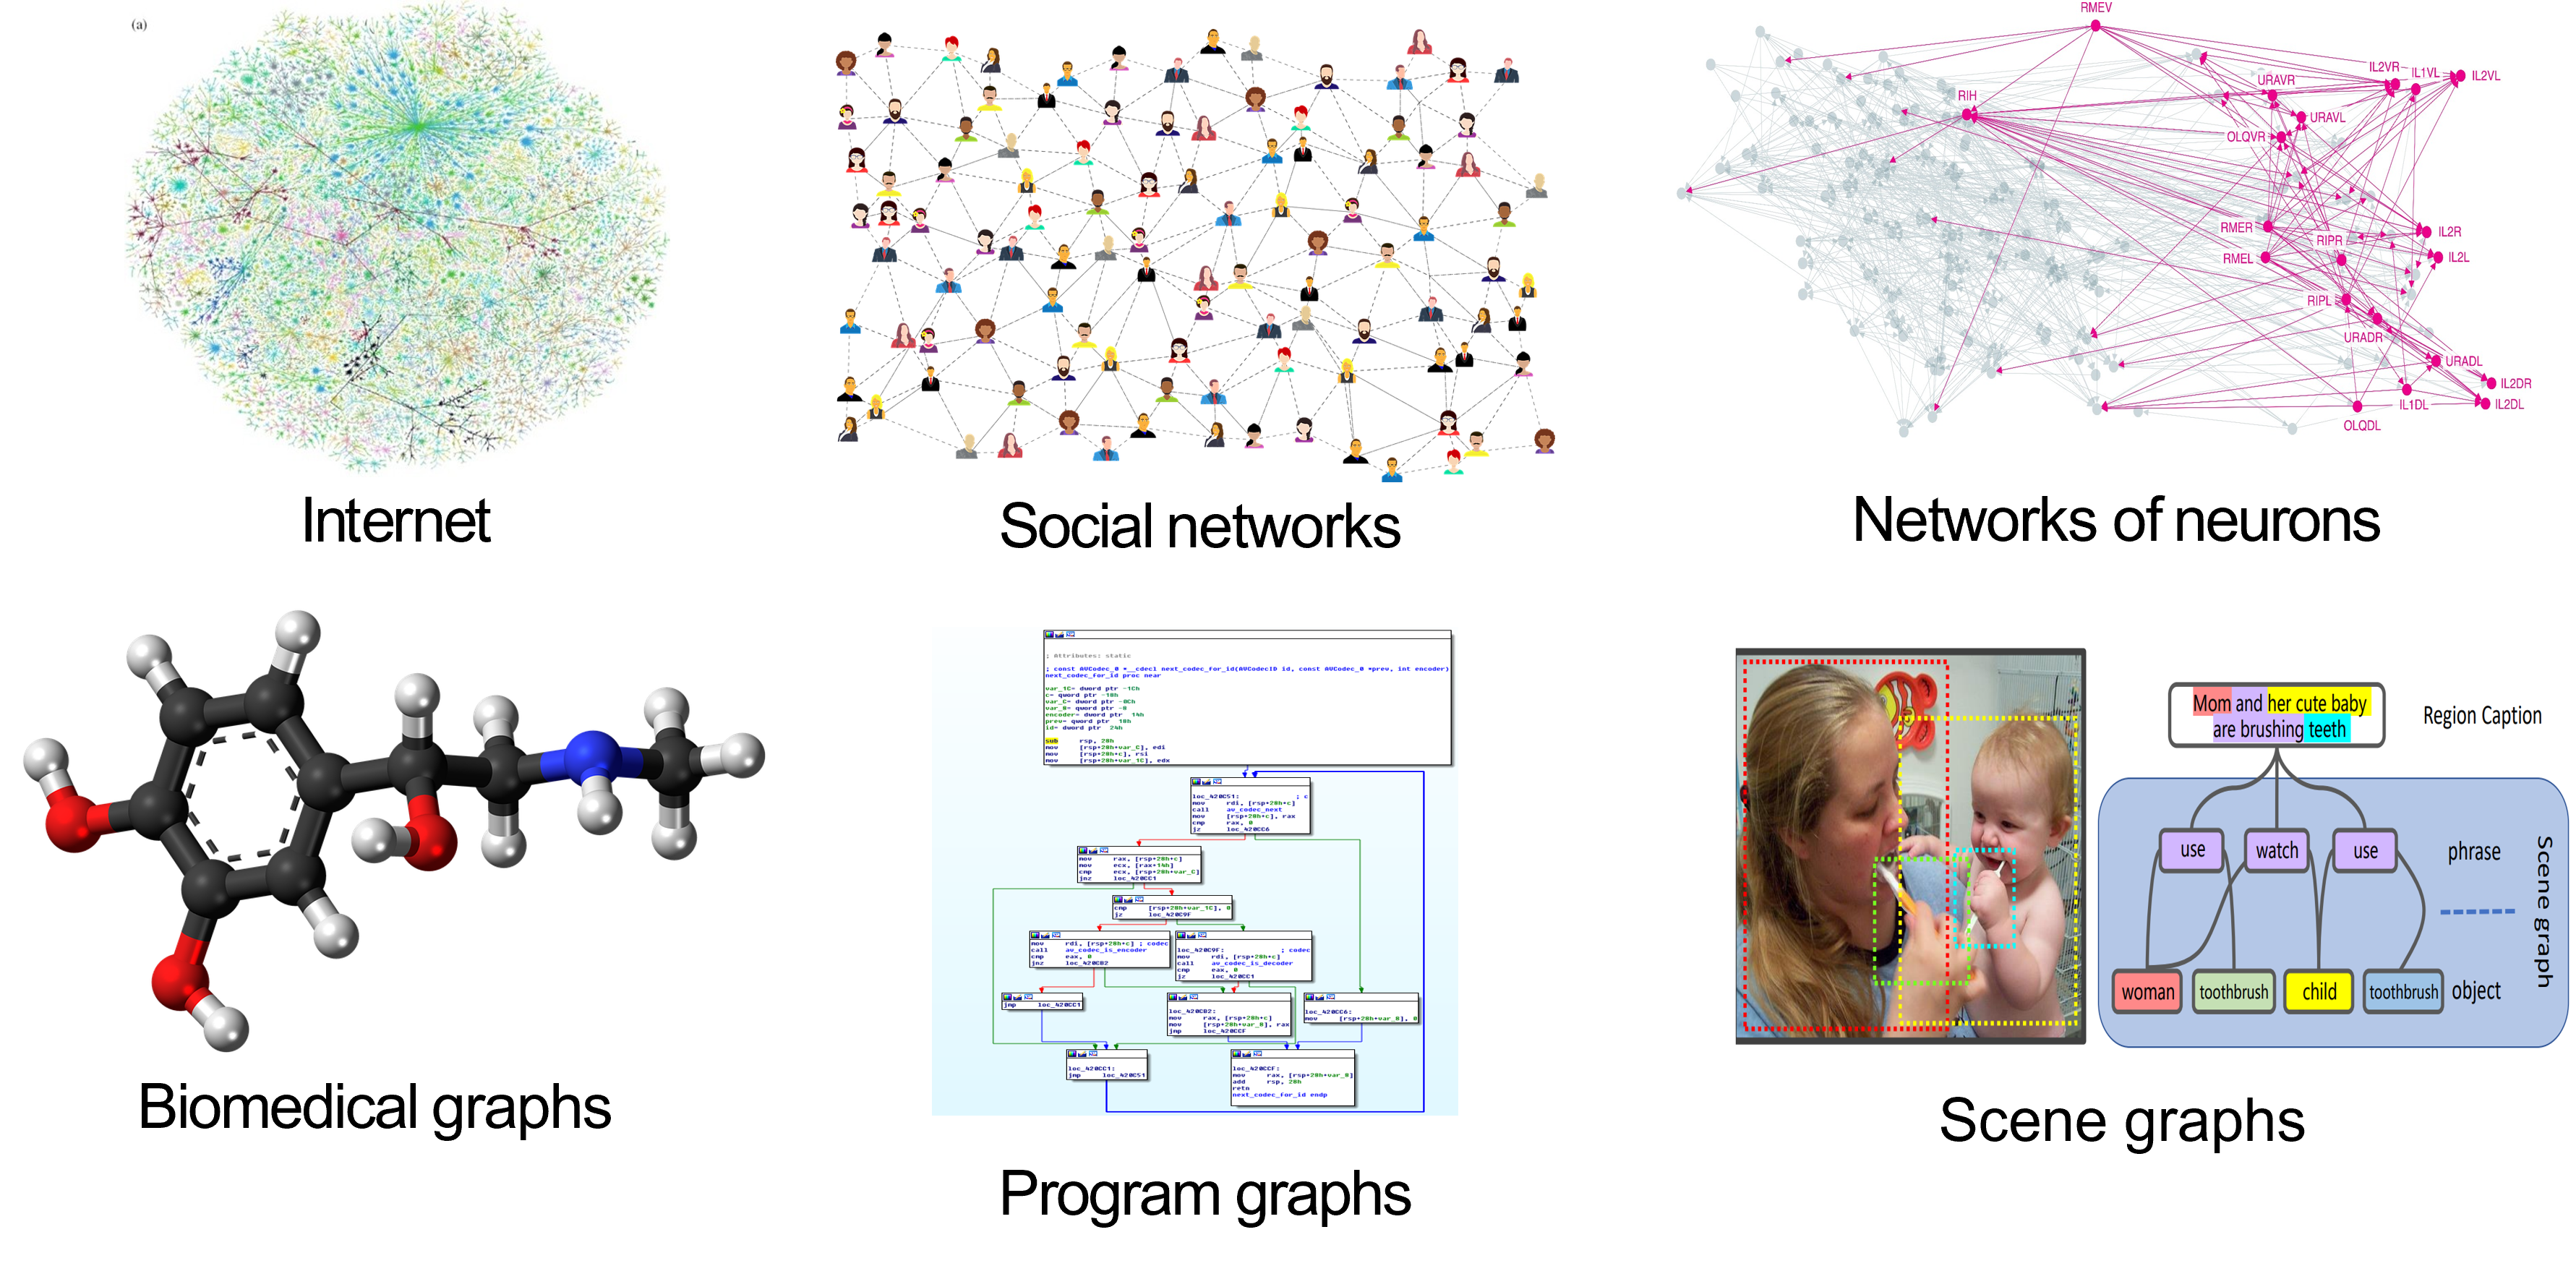
\includegraphics[width=\linewidth,keepaspectratio]{gnn1}
\end{center}	  

\end{frame}

%%%%%%%%%%%%%%%%%%%%%%%%%%%%%%%%%%%%%%%%%%%%%%%%%%%%%%%%%%%
\begin{frame}[fragile]\frametitle{}

\begin{center}
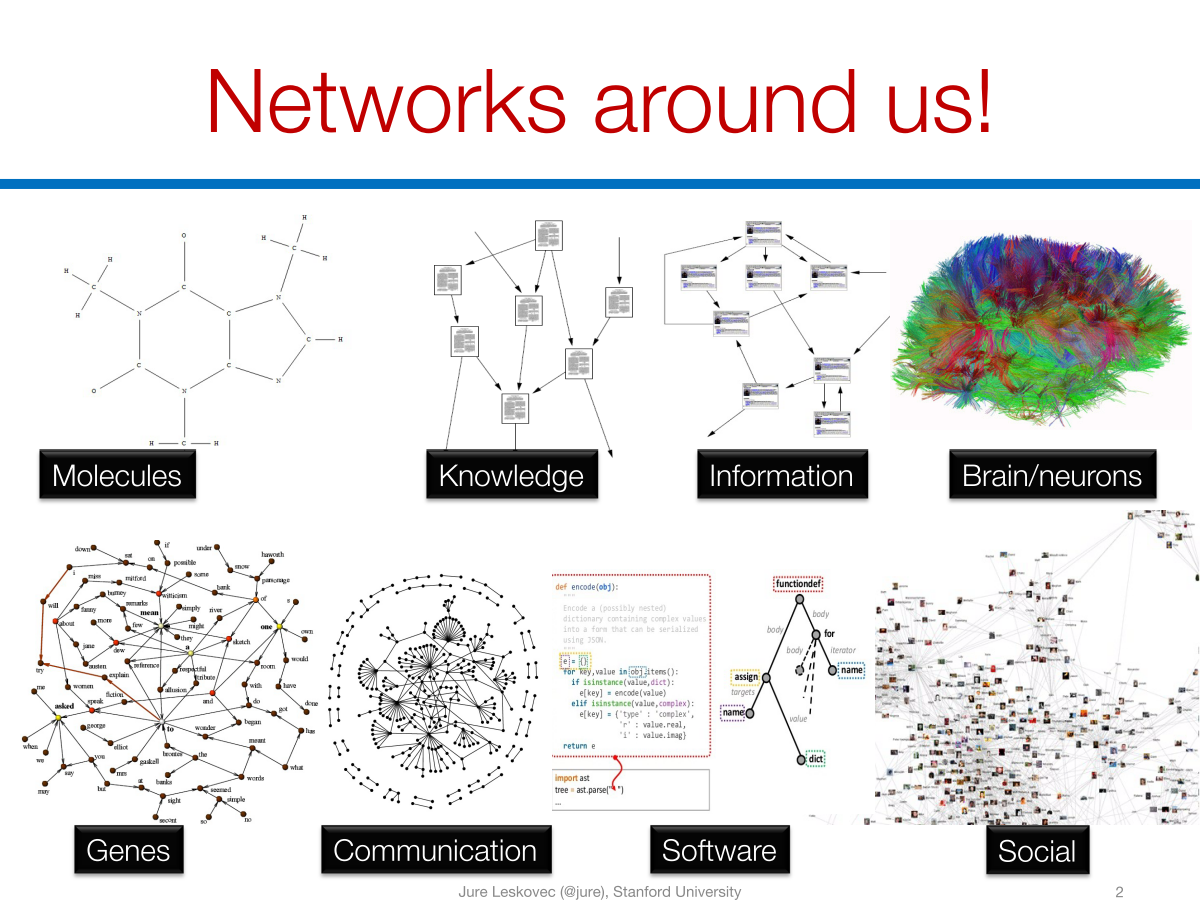
\includegraphics[width=\linewidth,keepaspectratio]{gnn2}
\end{center}	  

\end{frame}

%%%%%%%%%%%%%%%%%%%%%%%%%%%%%%%%%%%%%%%%%%%%%%%%%%%%%%%%%%%
\begin{frame}[fragile]\frametitle{}

\begin{center}
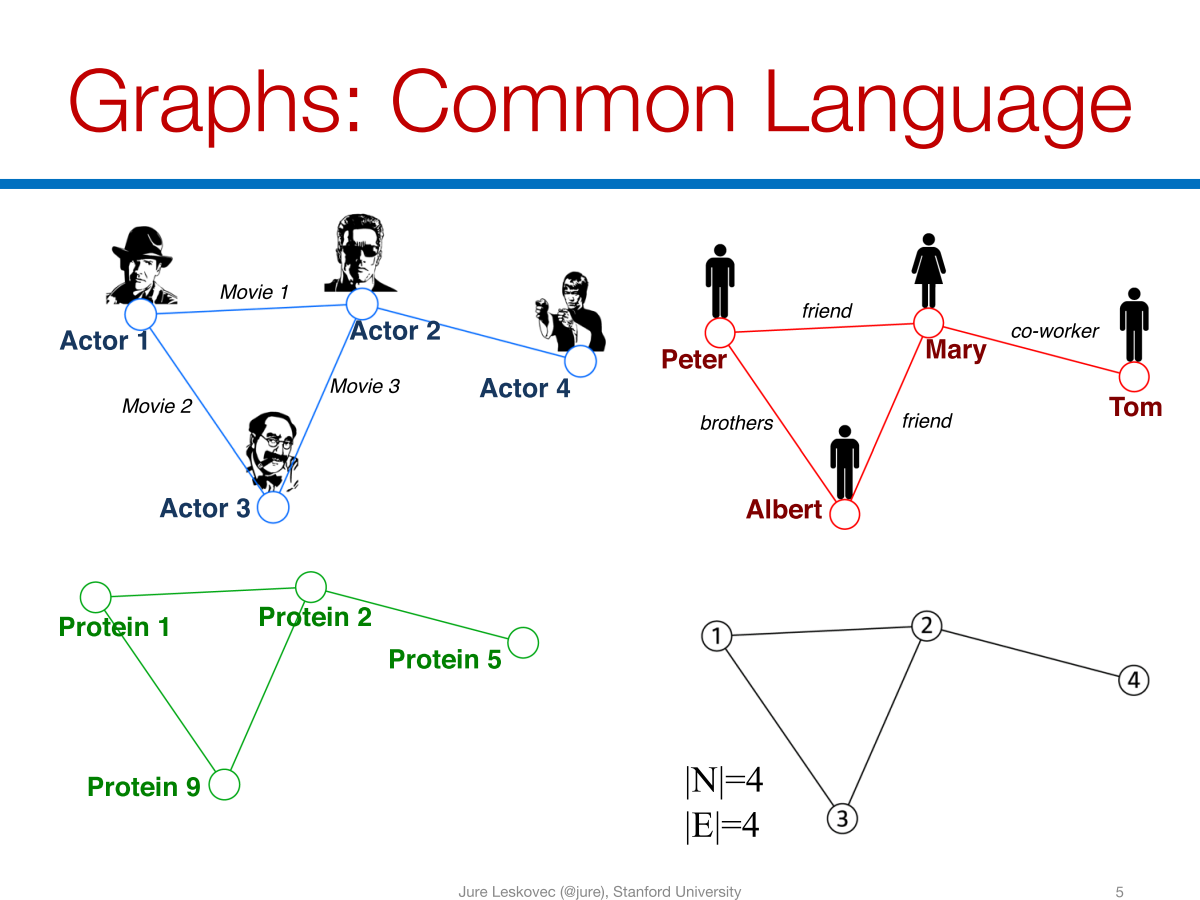
\includegraphics[width=\linewidth,keepaspectratio]{gnn3}
\end{center}	  

\end{frame}

%%%%%%%%%%%%%%%%%%%%%%%%%%%%%%%%%%%%%%%%%%%%%%%%%%%%%%%%%%%
\begin{frame}[fragile]\frametitle{Graphs: A Universal Language }

\begin{center}
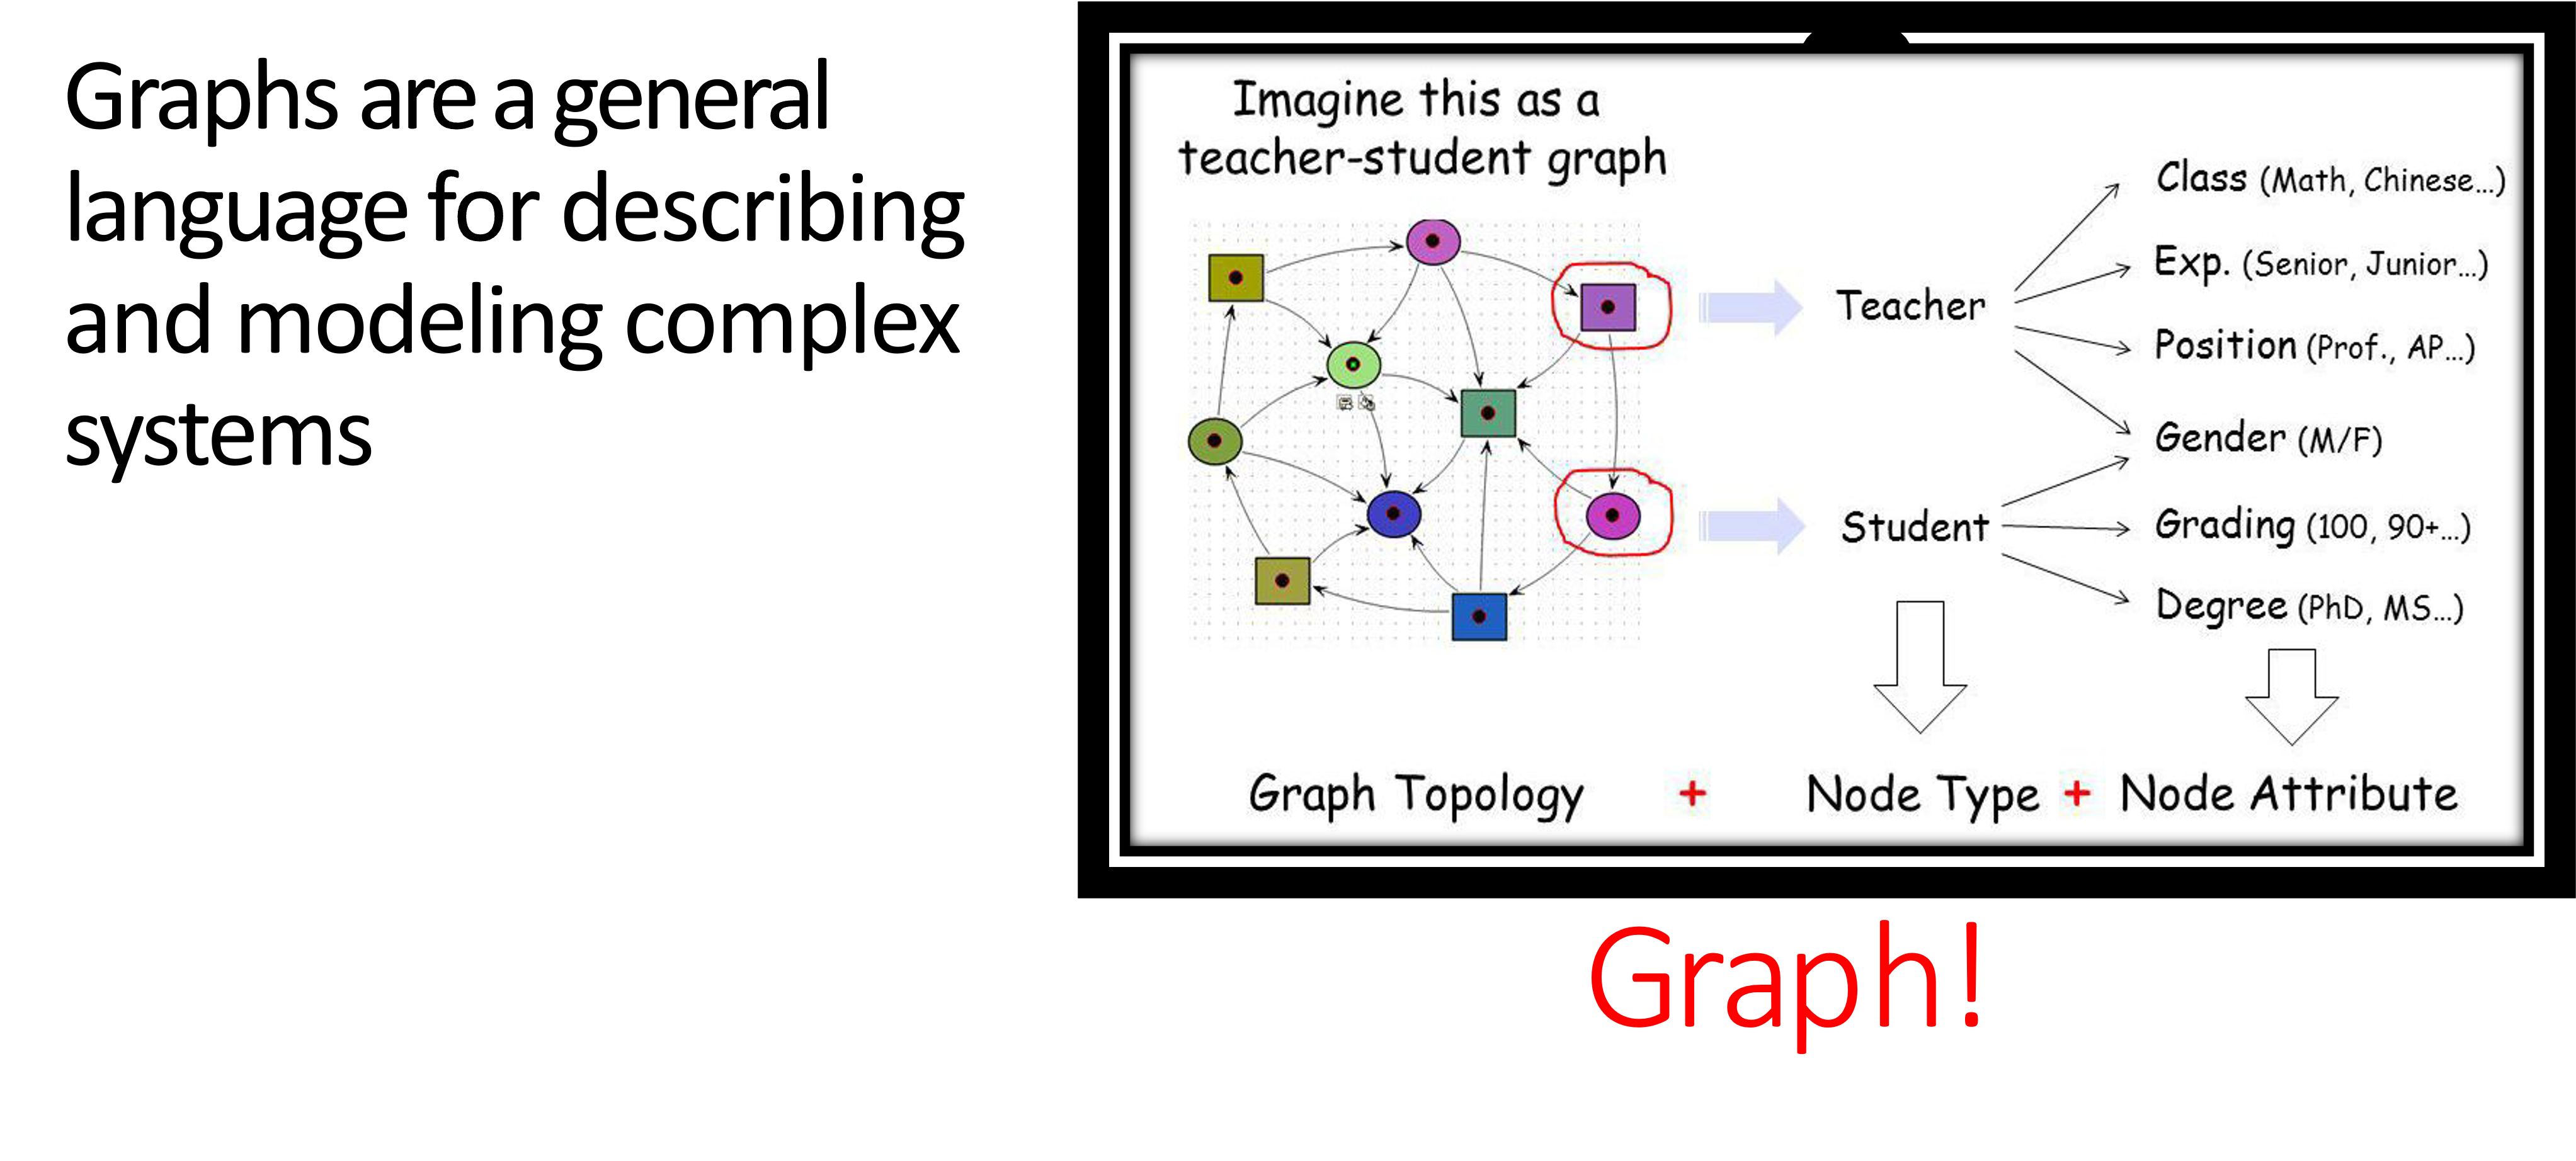
\includegraphics[width=\linewidth,keepaspectratio]{gnn4}
\end{center}	  

\end{frame}


%%%%%%%%%%%%%%%%%%%%%%%%%%%%%%%%%%%%%%%%%%%%%%%%%%%%%%%%%%%
\begin{frame}[fragile]\frametitle{Data as Graphs - Explicit }

\begin{center}
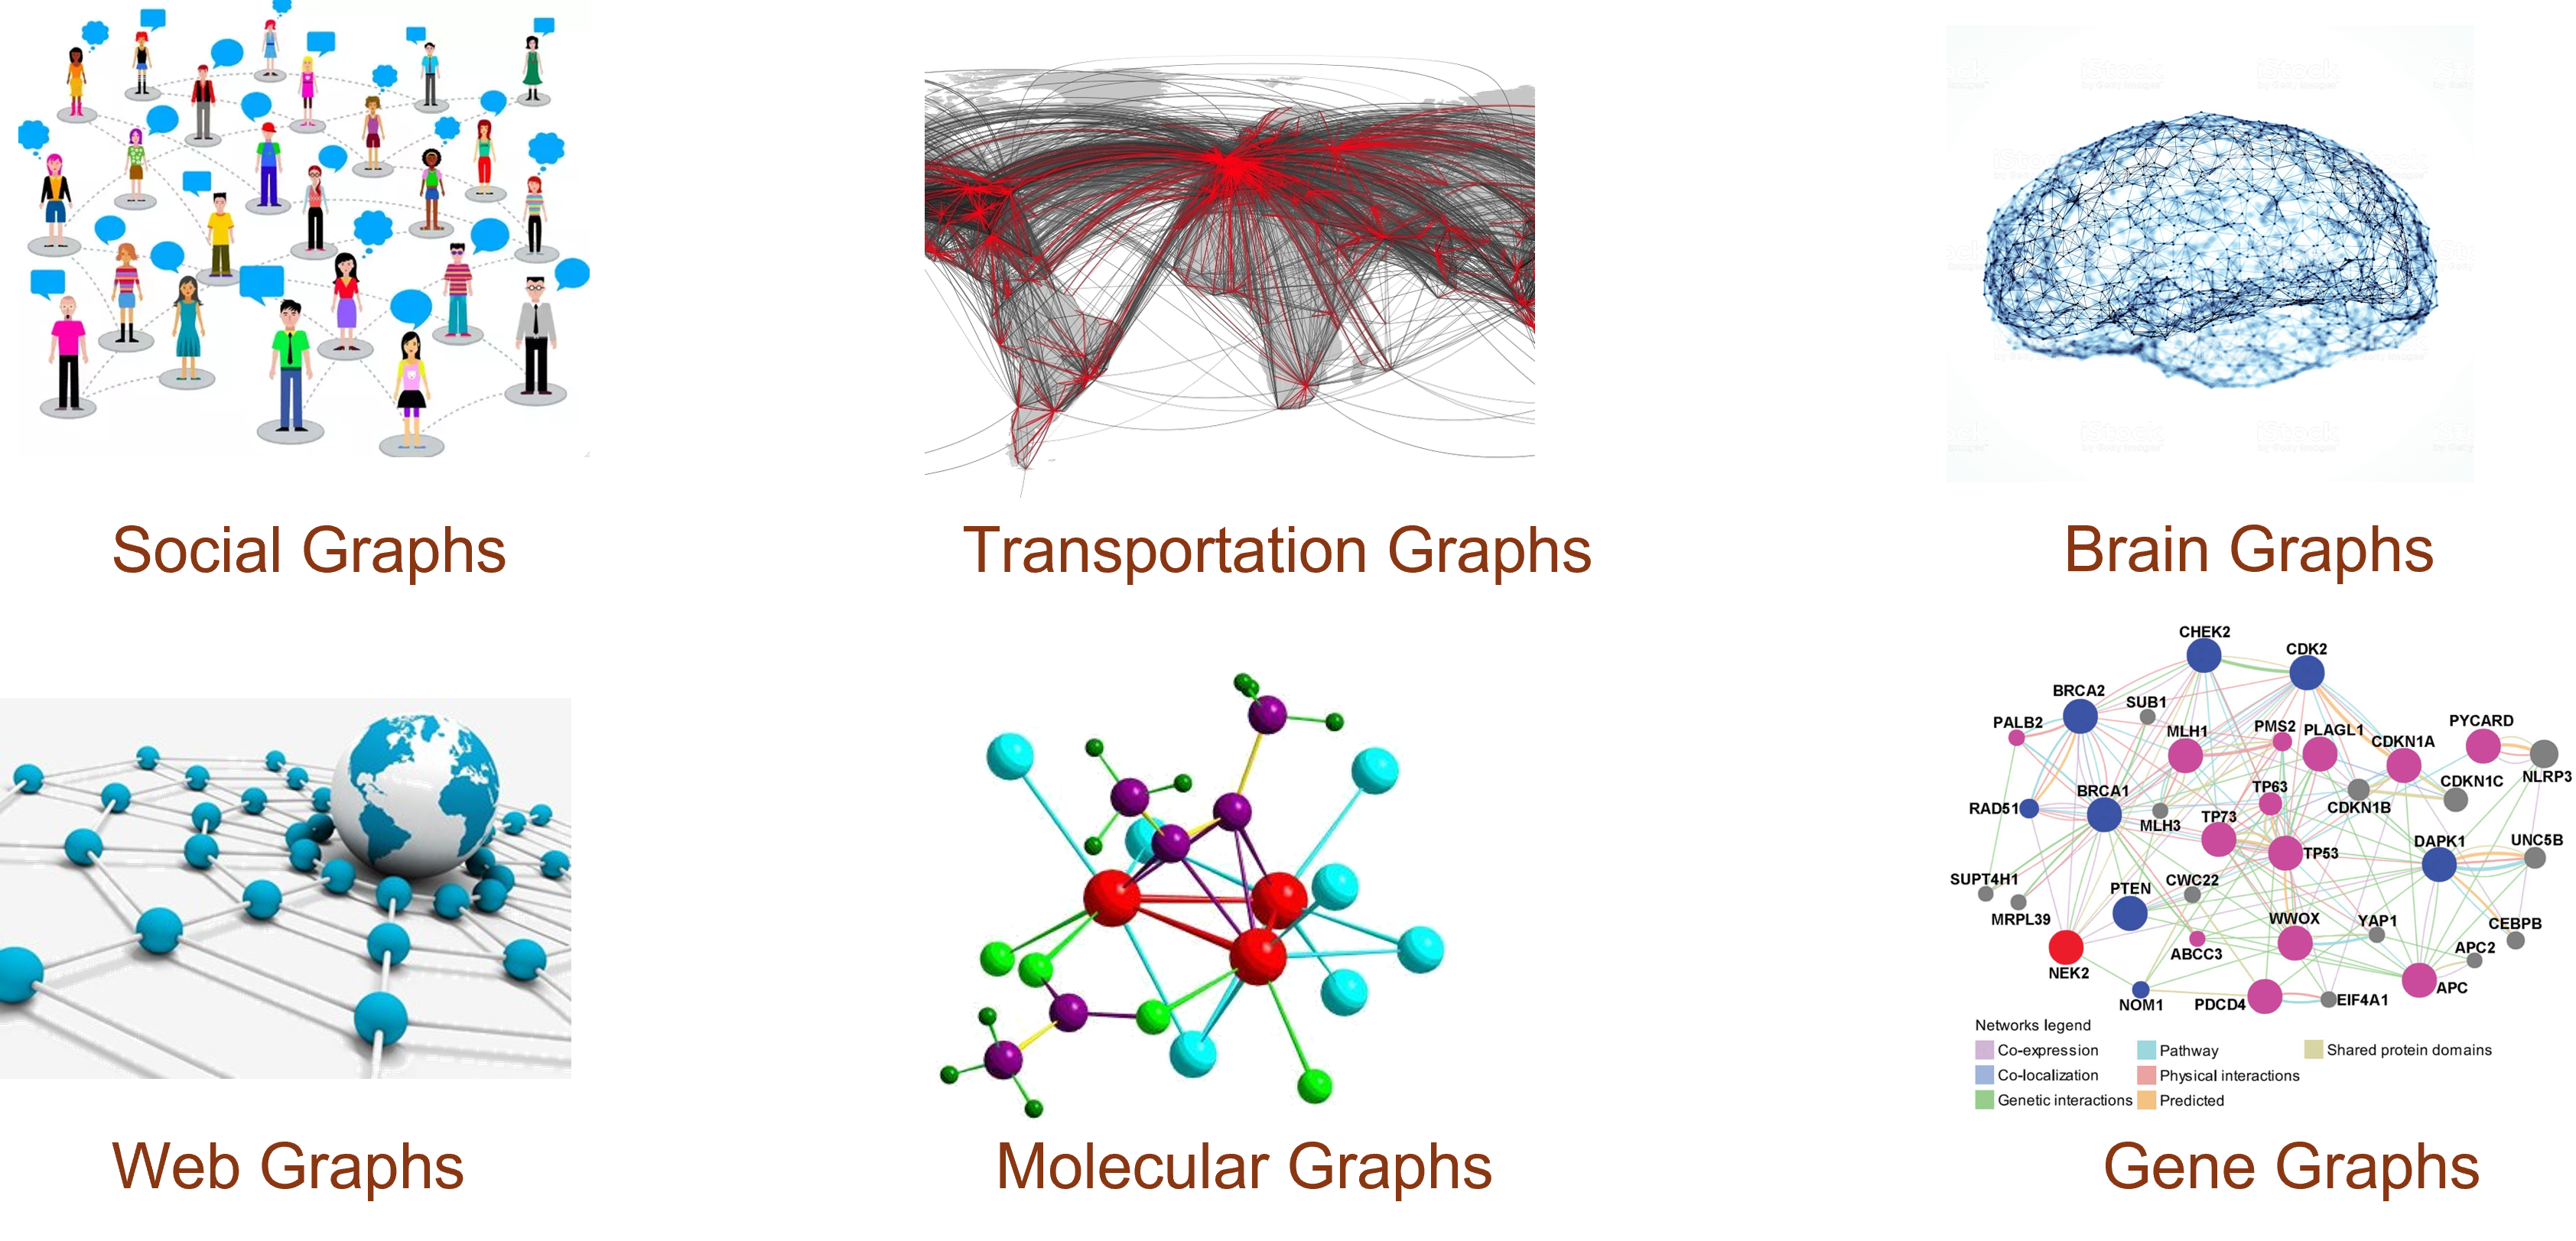
\includegraphics[width=\linewidth,keepaspectratio]{gnn5}
\end{center}	  

\end{frame}

%%%%%%%%%%%%%%%%%%%%%%%%%%%%%%%%%%%%%%%%%%%%%%%%%%%%%%%%%%%
\begin{frame}[fragile]\frametitle{Data as Graphs - Implicit }

\begin{center}
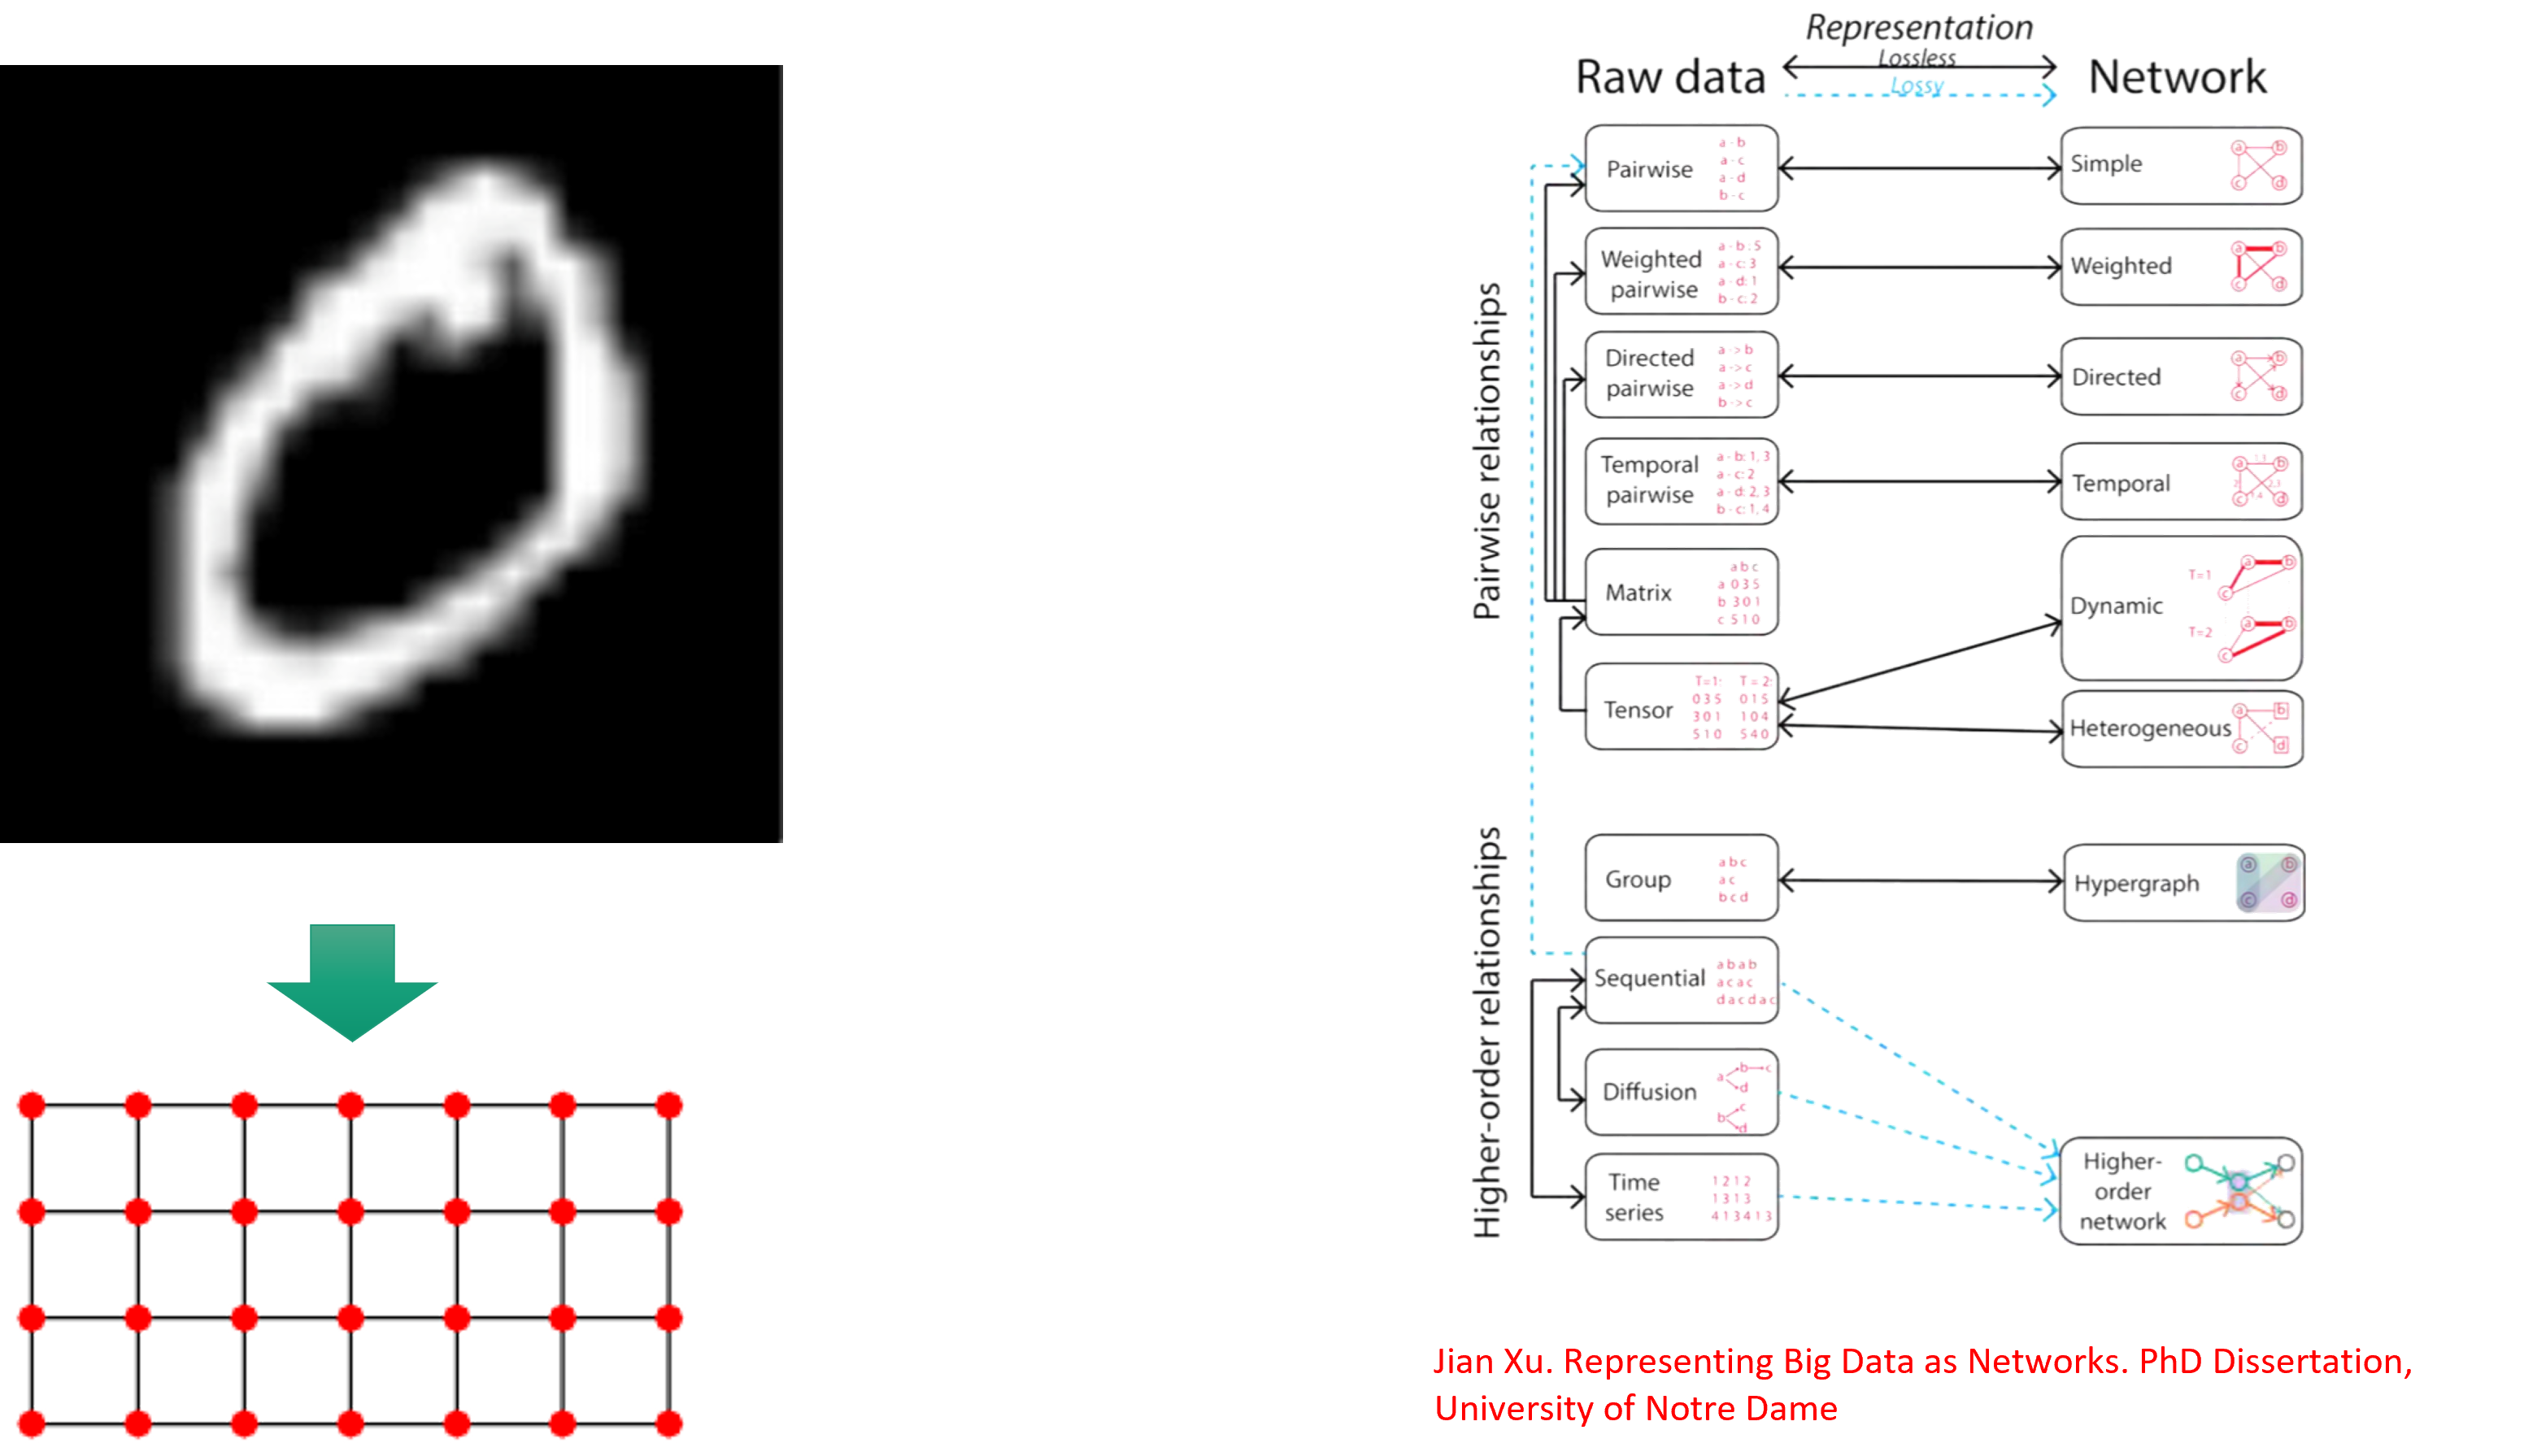
\includegraphics[width=\linewidth,keepaspectratio]{gnn6}
\end{center}	  

\end{frame}



%%%%%%%%%%%%%%%%%%%%%%%%%%%%%%%%%%%%%%%%%%%%%%%%%%%%%%%%%%%
\begin{frame}[fragile]\frametitle{}

\begin{center}
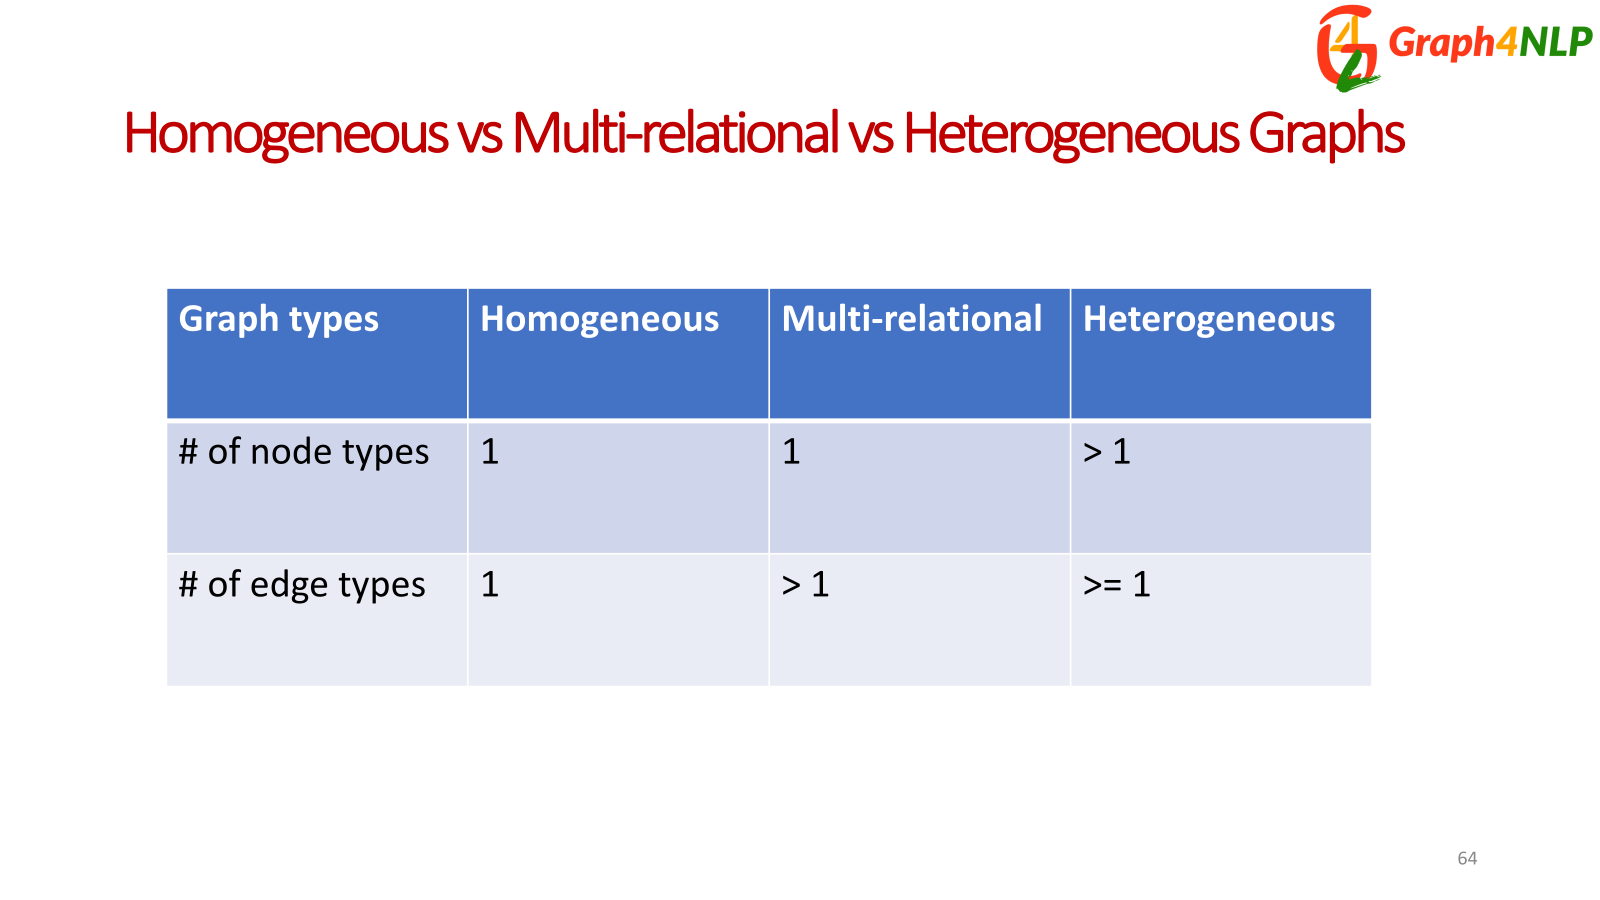
\includegraphics[width=\linewidth,keepaspectratio]{gnn8}
\end{center}	  

\end{frame}


%%%%%%%%%%%%%%%%%%%%%%%%%%%%%%%%%%%%%%%%%%%%%%%%%%%%%%%%%%%%%%%%%%%%%%%%%%%%%%%%%%
\begin{frame}\frametitle{Graph Components}

\begin{itemize}
\item Node (Vertex): A must data element for constructing a graph
\item Relationship (Edge) : Link between two nodes, can have direction and type.
\item Label: Node category/type such as PERSON, ORG, etc. One node can have many types.
\item Properties: Attributes or fields in Nodes or Edges, eg. A node can have Label PERSON and Property such as ``name: Jane''
\end{itemize}



{\tiny (Ref: Introduction to Neo4j - a hands-on crash course - neo4j)}
\end{frame}


%%%%%%%%%%%%%%%%%%%%%%%%%%%%%%%%%%%%%%%%%%%%%%%%%%%%%%%%%%%
\begin{frame}[fragile]\frametitle{Graphs and features}

\begin{center}
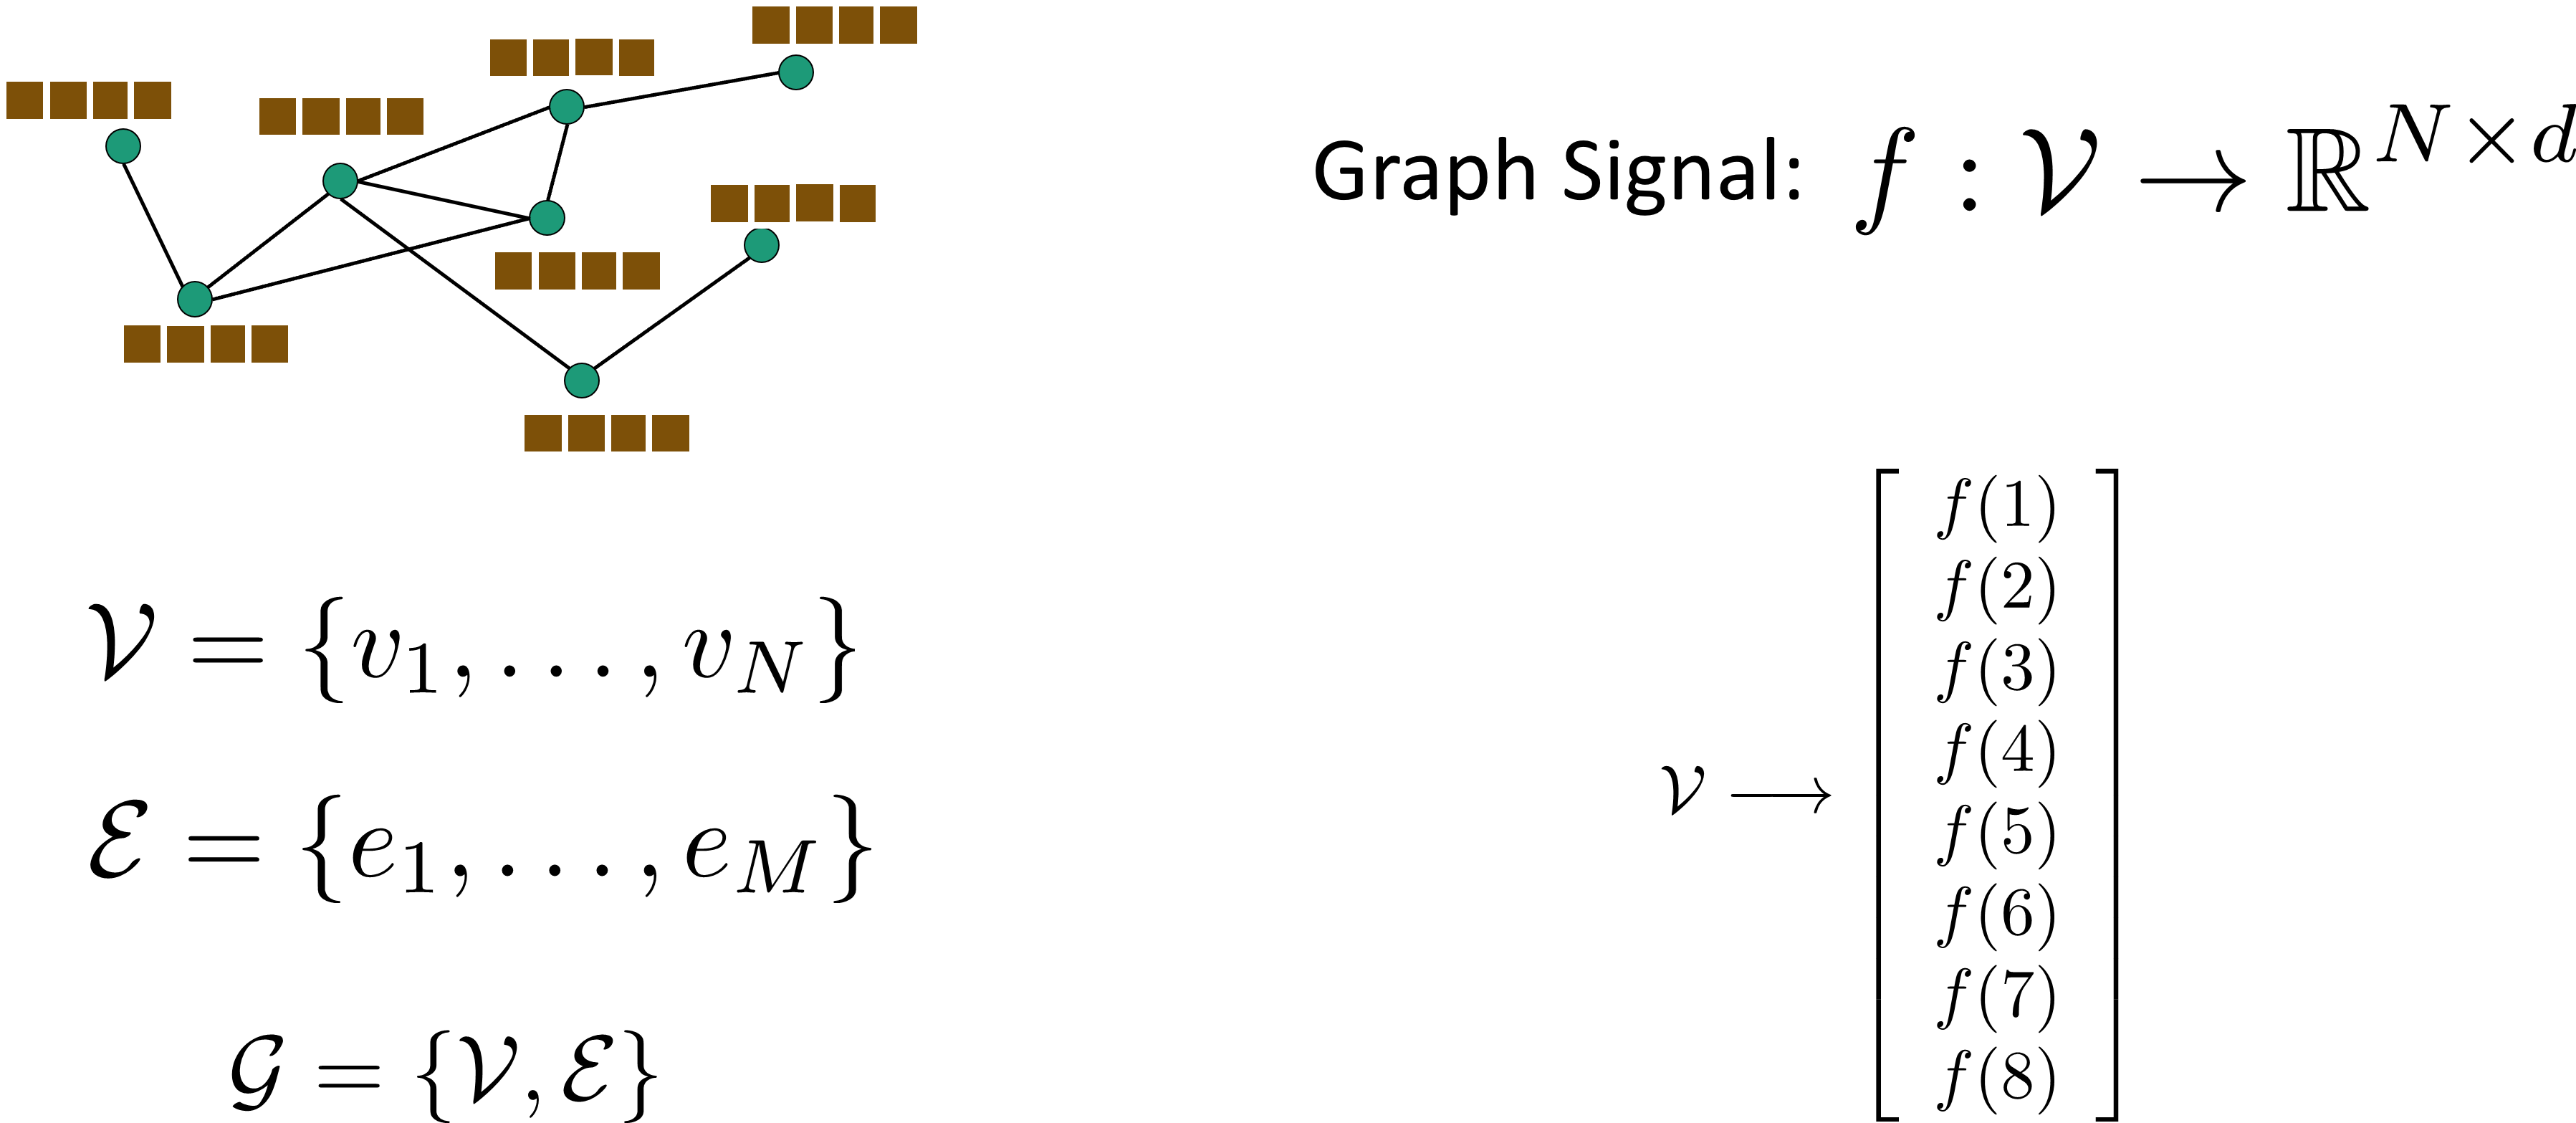
\includegraphics[width=\linewidth,keepaspectratio]{gnn9}
\end{center}	  

\end{frame}

%%%%%%%%%%%%%%%%%%%%%%%%%%%%%%%%%%%%%%%%%%%%%%%%%%%%%%%%%%%
\begin{frame}[fragile]\frametitle{Matrix Representations of Graphs}

\begin{center}
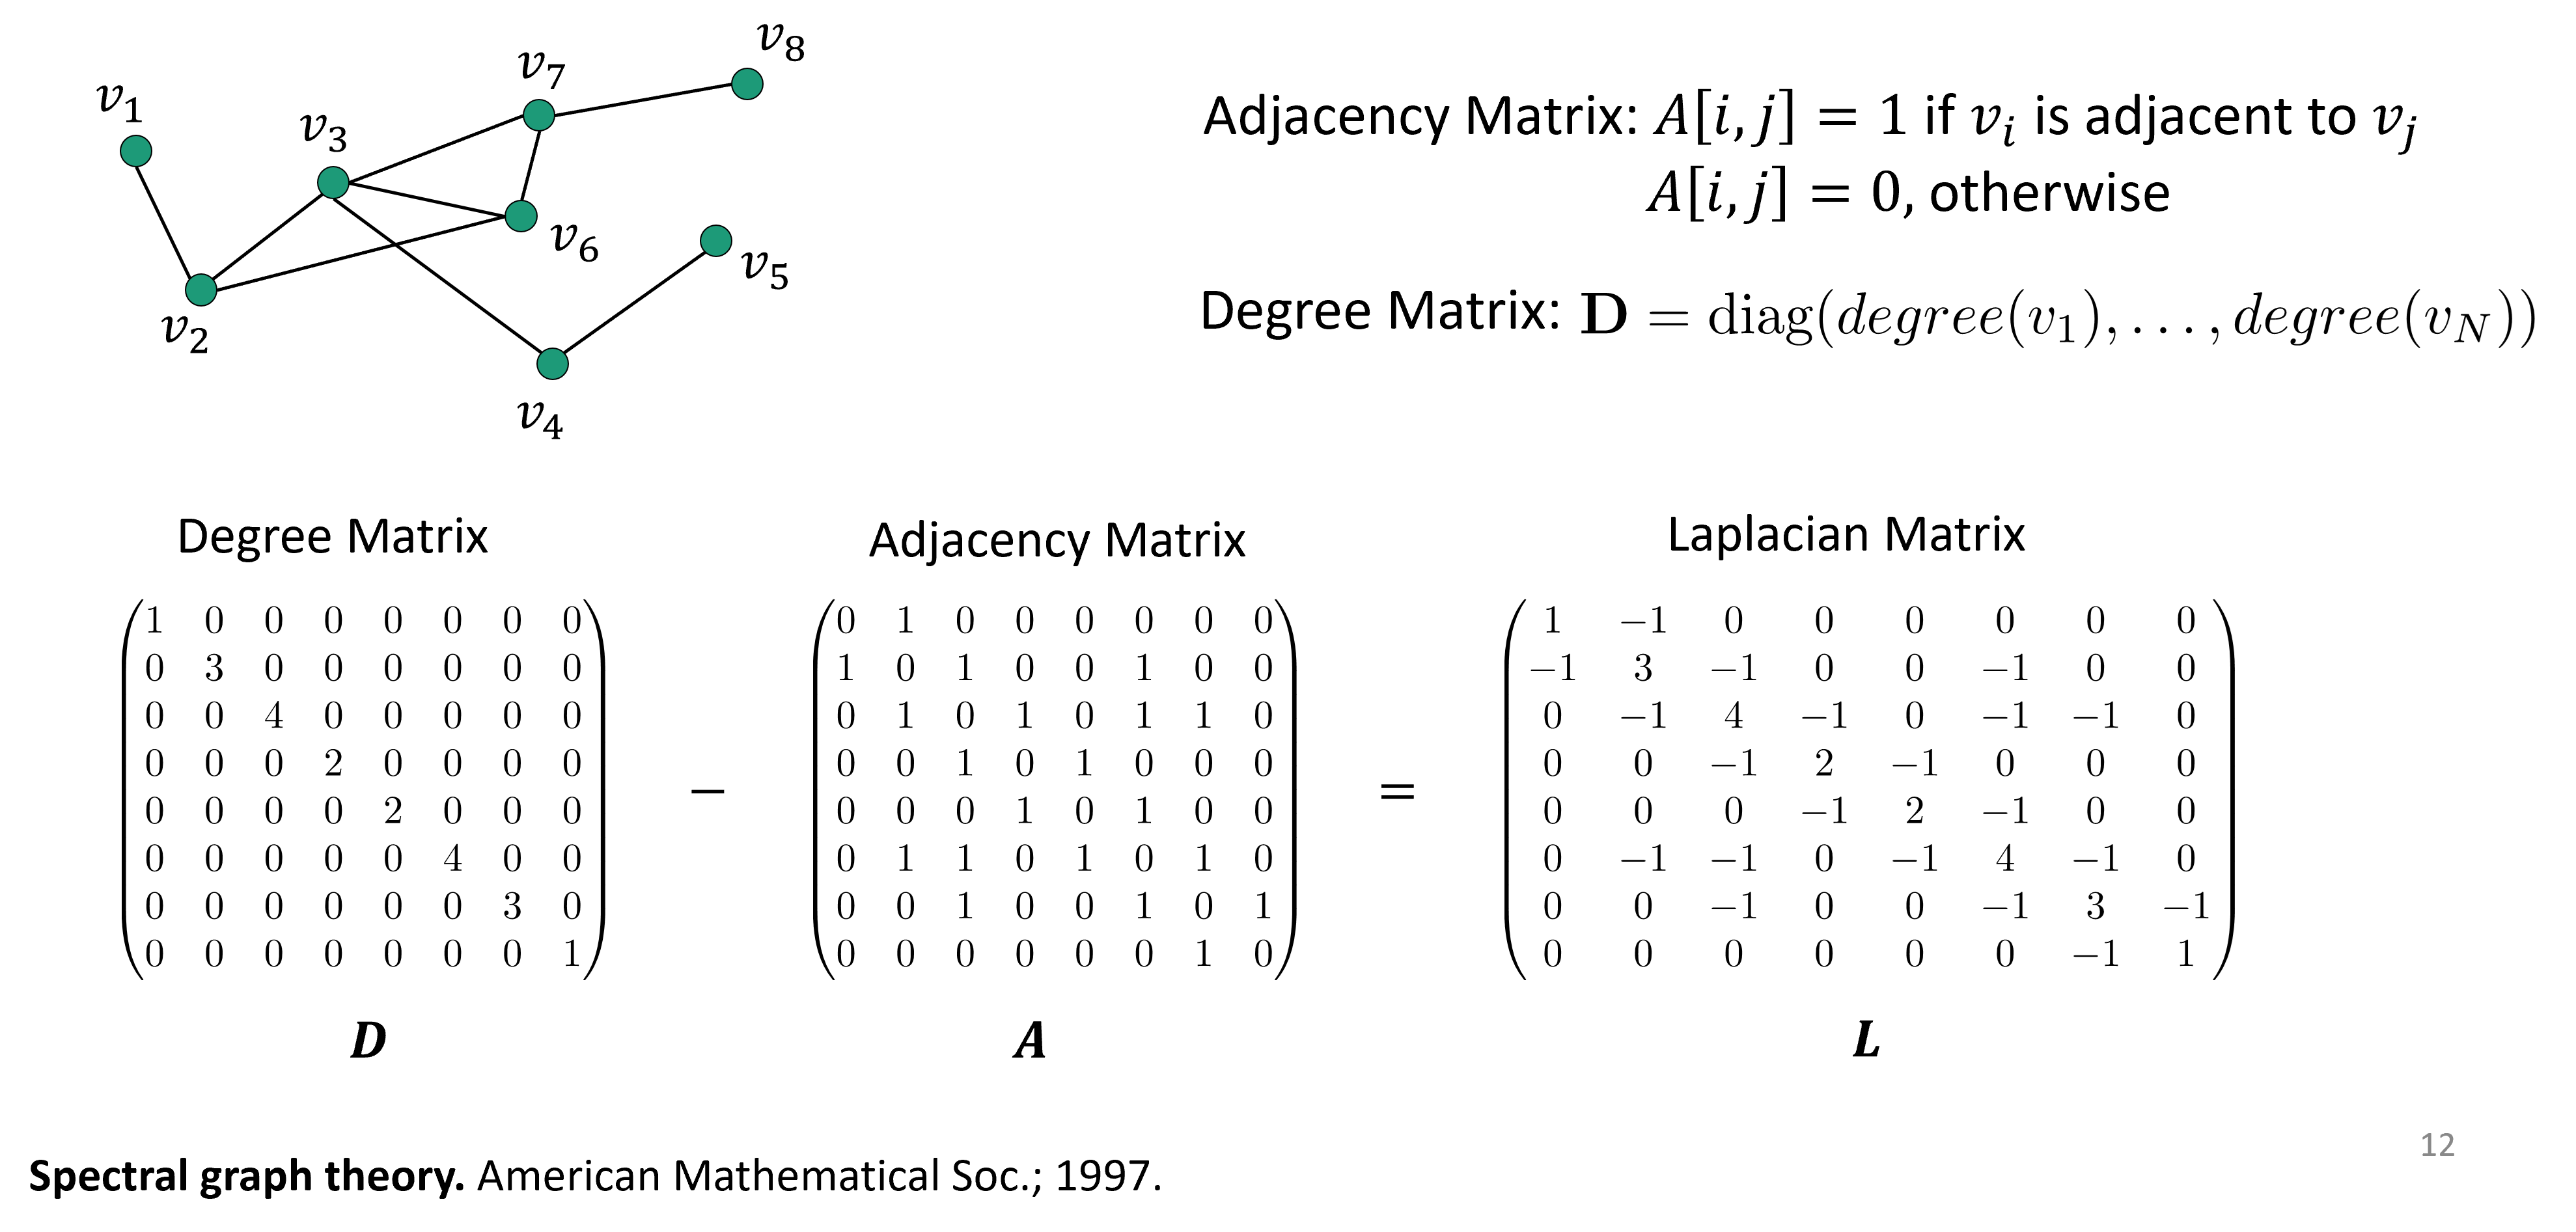
\includegraphics[width=\linewidth,keepaspectratio]{gnn10}
\end{center}	  

\end{frame}

%%%%%%%%%%%%%%%%%%%%%%%%%%%%%%%%%%%%%%%%%%%%%%%%%%%%%%%%%%%
\begin{frame}[fragile]\frametitle{Why Graphs? Why Now?}

\begin{itemize}
\item Universal language for describing complex data: Networks/graphs from science, nature, and technology are more similar than one would expect
\item Shared vocabulary between fields: Computer Science, Social science, Physics, Biology, Economics 
\item Data availability (+ computational challenges): Social/Internet, text, logic, program, bio, health, and medical
\item Impact: Social networking, Social media, Drug design, Event detection, Natural language processing, Computer vision, and Logic reasoning
\end{itemize}

\end{frame}

%%%%%%%%%%%%%%%%%%%%%%%%%%%%%%%%%%%%%%%%%%%%%%%%%%%%%%%%%%%%%%%%%%%%%%%%%%%%%%%%%%
\begin{frame}\frametitle{Identifying good Graph scenarios - 1/4}

Does the problem involve understanding relationships between entities?

Behavioral analysis:

\begin{center}
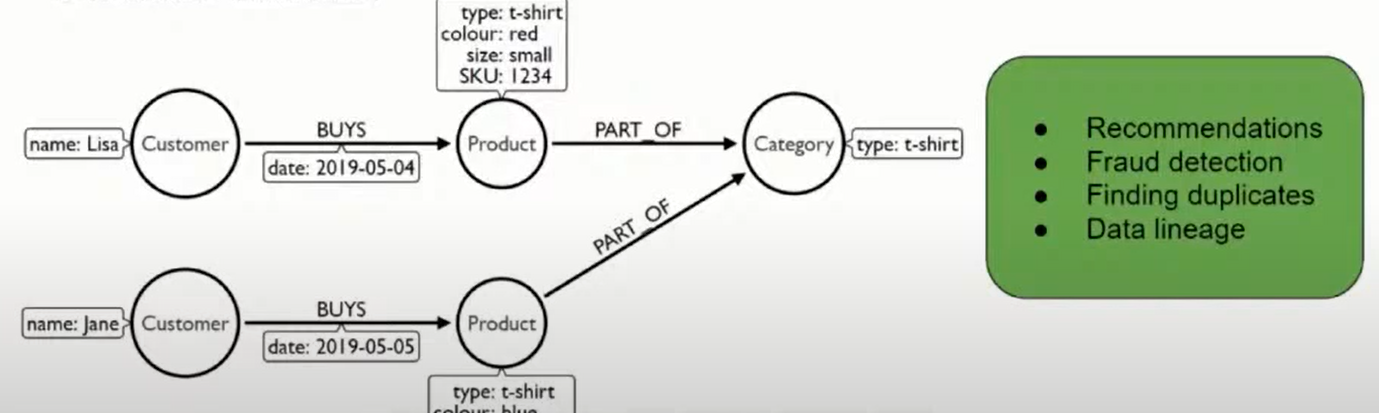
\includegraphics[width=\linewidth,keepaspectratio]{neo4j5}
\end{center}	  

{\tiny (Ref: Introduction to Neo4j - a hands-on crash course - neo4j)}
\end{frame}

%%%%%%%%%%%%%%%%%%%%%%%%%%%%%%%%%%%%%%%%%%%%%%%%%%%%%%%%%%%%%%%%%%%%%%%%%%%%%%%%%%
\begin{frame}\frametitle{Identifying good Graph scenarios - 2/4}

Does the problem involve a lot of self-referencing to the same type of entity?

Org chart of employees:

\begin{center}
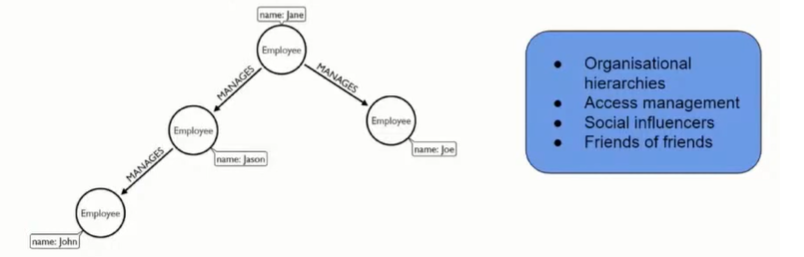
\includegraphics[width=\linewidth,keepaspectratio]{neo4j6}
\end{center}	  

{\tiny (Ref: Introduction to Neo4j - a hands-on crash course - neo4j)}
\end{frame}

%%%%%%%%%%%%%%%%%%%%%%%%%%%%%%%%%%%%%%%%%%%%%%%%%%%%%%%%%%%%%%%%%%%%%%%%%%%%%%%%%%
\begin{frame}\frametitle{Identifying good Graph scenarios - 3/4}

Does the problem explore relationships of varying and unknown depth?

Changes in manufacturing process:

\begin{center}
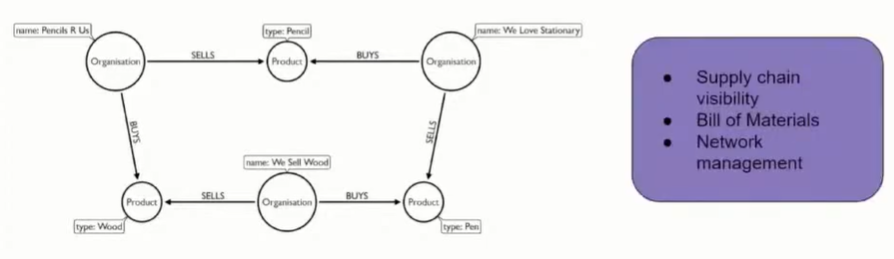
\includegraphics[width=\linewidth,keepaspectratio]{neo4j7}
\end{center}	  

{\tiny (Ref: Introduction to Neo4j - a hands-on crash course - neo4j)}
\end{frame}

%%%%%%%%%%%%%%%%%%%%%%%%%%%%%%%%%%%%%%%%%%%%%%%%%%%%%%%%%%%%%%%%%%%%%%%%%%%%%%%%%%
\begin{frame}\frametitle{Identifying good Graph scenarios - 4/4}

Does the problem involve discovering lots of different routes or paths?

Optimum logistics:

\begin{center}
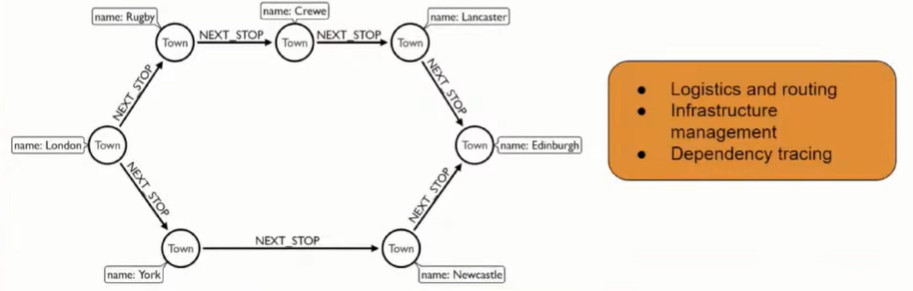
\includegraphics[width=\linewidth,keepaspectratio]{neo4j8}
\end{center}	  

{\tiny (Ref: Introduction to Neo4j - a hands-on crash course - neo4j)}
\end{frame}

